\documentclass[a4paper, 11pt]{article}
\usepackage[portuguese]{babel}
\usepackage{style}
\usepackage{subfig}

\title{\Huge Projecto POO 2024\\
        \it \huge POO Financial Systems
}
\author{Vasco Guilherme Alves, nº 2022228207\\
Miguel Angelo Silva, nº 2023221244\\
}
\date{Programação Orientada a Objectos --- LEI 2024}

\newcommand\ssection[1]{\section{#1} }
\newcommand\sssection[1]{ \subsection*{\color{MidnightBlue}#1}\vspace{-2ex} }

\begin{document}
\maketitle
\tableofcontents

\newpage
\ssection{Introdução}

O presente trabalho propõe o desenvolvimento de uma aplicação de gestão financeira, designada \textit{POO Financial Services} (POOFS), com o objetivo de permitir a uma empresa registar e emitir faturas aos seus clientes. Estas faturas devem conter produtos de dois tipos: alimentares e de farmácia, que diferem nas suas categorias, certificações, se são prescritos e nos cálculos da taxa IVA.

Por fim, a aplicação deverá oferecer uma interface eficiente e intuitiva, permitindo aos utilizadores a inserção e consulta de dados, bem como a exportação e importação através de ficheiros.

\ssection{Manual do Utilizador}

\sssection{Início do Programa}
Para começar a usar o programa:
\begin{enumerate}
    \item Certifique-se de que os ficheiros \texttt{dados.ser} ou \texttt{dados-iniciais.txt} estão no mesmo diretório do programa (caso existam).
    \item Compile e execute o ficheiro \texttt{POOFS.java}.
    \item O programa irá carregar os dados guardados anteriormente (se disponíveis) e mostrar o menu principal.
\end{enumerate}

\sssection{Menu Principal}
O menu principal oferece várias opções que cobrem as principais funcionalidades da aplicação:
\begin{enumerate}
    \item \textbf{Criar/Editar Cliente}: Cria ou edita informações de clientes.
    \item \textbf{Listar Clientes}: Mostra todos os clientes registados.
    \item \textbf{Criar/Editar Fatura}: Cria ou atualiza faturas associadas a clientes.
    \item \textbf{Listar Faturas}: Exibe todas as faturas emitidas.
    \item \textbf{Consultar Fatura}: Permite ver os detalhes de uma fatura específica.
    \item \textbf{Importar Faturas}: Carrega dados de clientes e faturas a partir de ficheiros externos.
    \item \textbf{Exportar Faturas}: Grava os dados de clientes num ficheiro de texto.
    \item \textbf{Estatísticas}: Apresenta dados gerais sobre clientes, faturas e produtos.
    \item \textbf{Sair}: Guarda os dados e fecha o programa.
\end{enumerate}

\ssection{Funcionalidades em Detalhe}
\textbf{Criar/Editar Cliente} --- Mostra um menu que permite criar ou editar clientes. Se escolher criar um cliente novo vai pedir o nome do cliente e as restantes informações. Caso já exista um cliente com o nome inserido permite ao utilizador escolher editar esse cliente. Se escolher a segunda opção, editar, será mostrada um menu com todos os clientes onde pode escolher qual editar.

\textbf{Listar Clientes} --- É impressa a listagem de todos os clientes.

\textbf{Criar/Editar Fatura} --- Mostra um menu onde escolhe-se o cliente a que diz respeito a fatura, depois o utilizador pode escolher entre criar uma fatura nova para esse cliente ou editar uma das faturas já existentes. No mesmo modo que a primeira opção, o utilizador pode escolher editar uma fatura que já existe se ao criar inserir um ID que já existe. Ao editar a fatura, podemos também adicionar e remover produtos novos.

\textbf{Listar Faturas} --- São apresentadas todas as faturas de todos os clientes registados, incluindo toda a informação que diz respeito aos produtos, incluindo o IVA, o total da fatura, a ainda informação sobre o cliente e a data.  

\textbf{Consultar Fatura} --- Permite consultar uma fatura especifica- Mostra todas as informações de uma fatura, incluindo o total com e sem IVA.

\textbf{Importar Faturas} --- Carrega dados de um ficheiro indicado pelo utilizador, em formato de texto ou serializado.

\textbf{Exportar Faturas} --- Permite gravar os dados de clientes num ficheiro para facilitar backups e consultas externas.

\textbf{Estatísticas} --- Apresenta o total de clientes registados, o número de faturas emitidas, os produtos listados e os valores dos produtos faturados (com e sem IVA).

\textbf{Sair} --- Guarda os dados no ficheiro \texttt{dados.ser} e termina o programa.

\ssection{Mapa de Classes}
\sssection{Estrutura Geral (\textit{Packages})}
O programa está dividido em três pacotes principais:
\begin{itemize}
    \item \textbf{produto}: Contém classes relacionadas aos clientes, faturas e todos os tipos produtos.
    \item \textbf{gestao}: Responsável pela gestão de clientes, faturas e produtos. Isto inclui a criação, edição, remoção e a listagem dos itens de cada cada gestor.
    \item \textbf{io}: Inclui classes utilitárias para entrada e validação de dados do utilizador tal como a importação e exportação de ficheiros.
\end{itemize}

\sssection{Descrição das Classes}
\begin{itemize}
    \setlength\itemsep{0em}
    \item \textbf{{POOFS}}: Classe principal que gere o menu e as operações principais.
    \item \textbf{{Cliente}}: Armazena informações de clientes e as suas faturas.
    \item \textbf{{Fatura}}: Representa uma fatura emitida, com uma lista de produtos.
    \item \textbf{{Produto}}: Classe genérica para produtos.
    \item \textbf{{ProdutoAlimentar}}: Subclasse de \texttt{Produto}, dividida em categorias baseadas na taxa de IVA.
    \item \textbf{{ProdutoFarmacia}}: Subclasse de \texttt{Produto} para produtos farmacêuticos.
    \item \textbf{GestorClientes}, \textbf{GestorFaturas} e \textbf{GestorProdutos}: Gerem a lógica das respetivas entidades.
    \item \textbf{{Leitor}}: Facilita a entrada e validação de dados pelo utilizador.
    \item \textbf{{FicheiroIO}}: Gere importação e exportação de dados.
\end{itemize}

\ssection{UML}

\begin{figure}[h!]
    \centering
    \subfloat[\centering UML Projetado]{{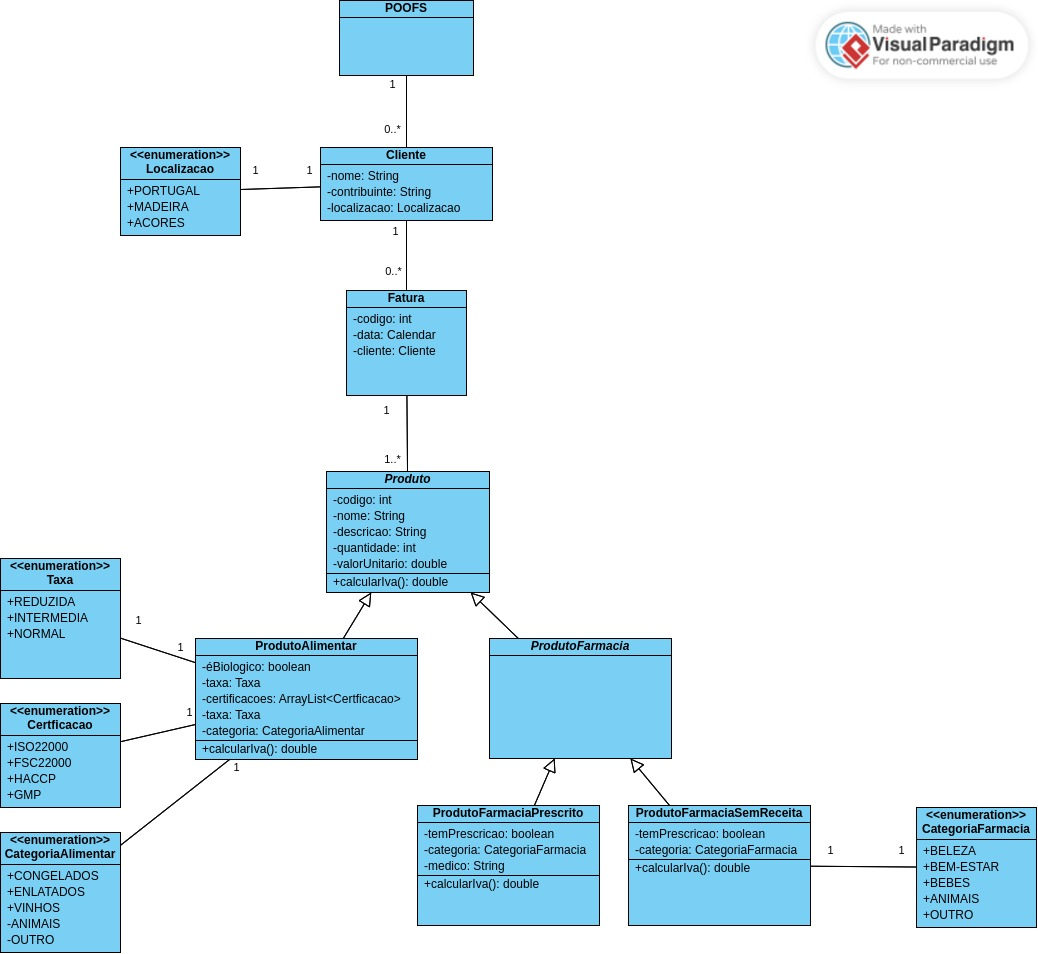
\includegraphics[width=0.45\textwidth]{uml-1} }}%
    \qquad
    \subfloat[\centering UML do Projecto Final]{{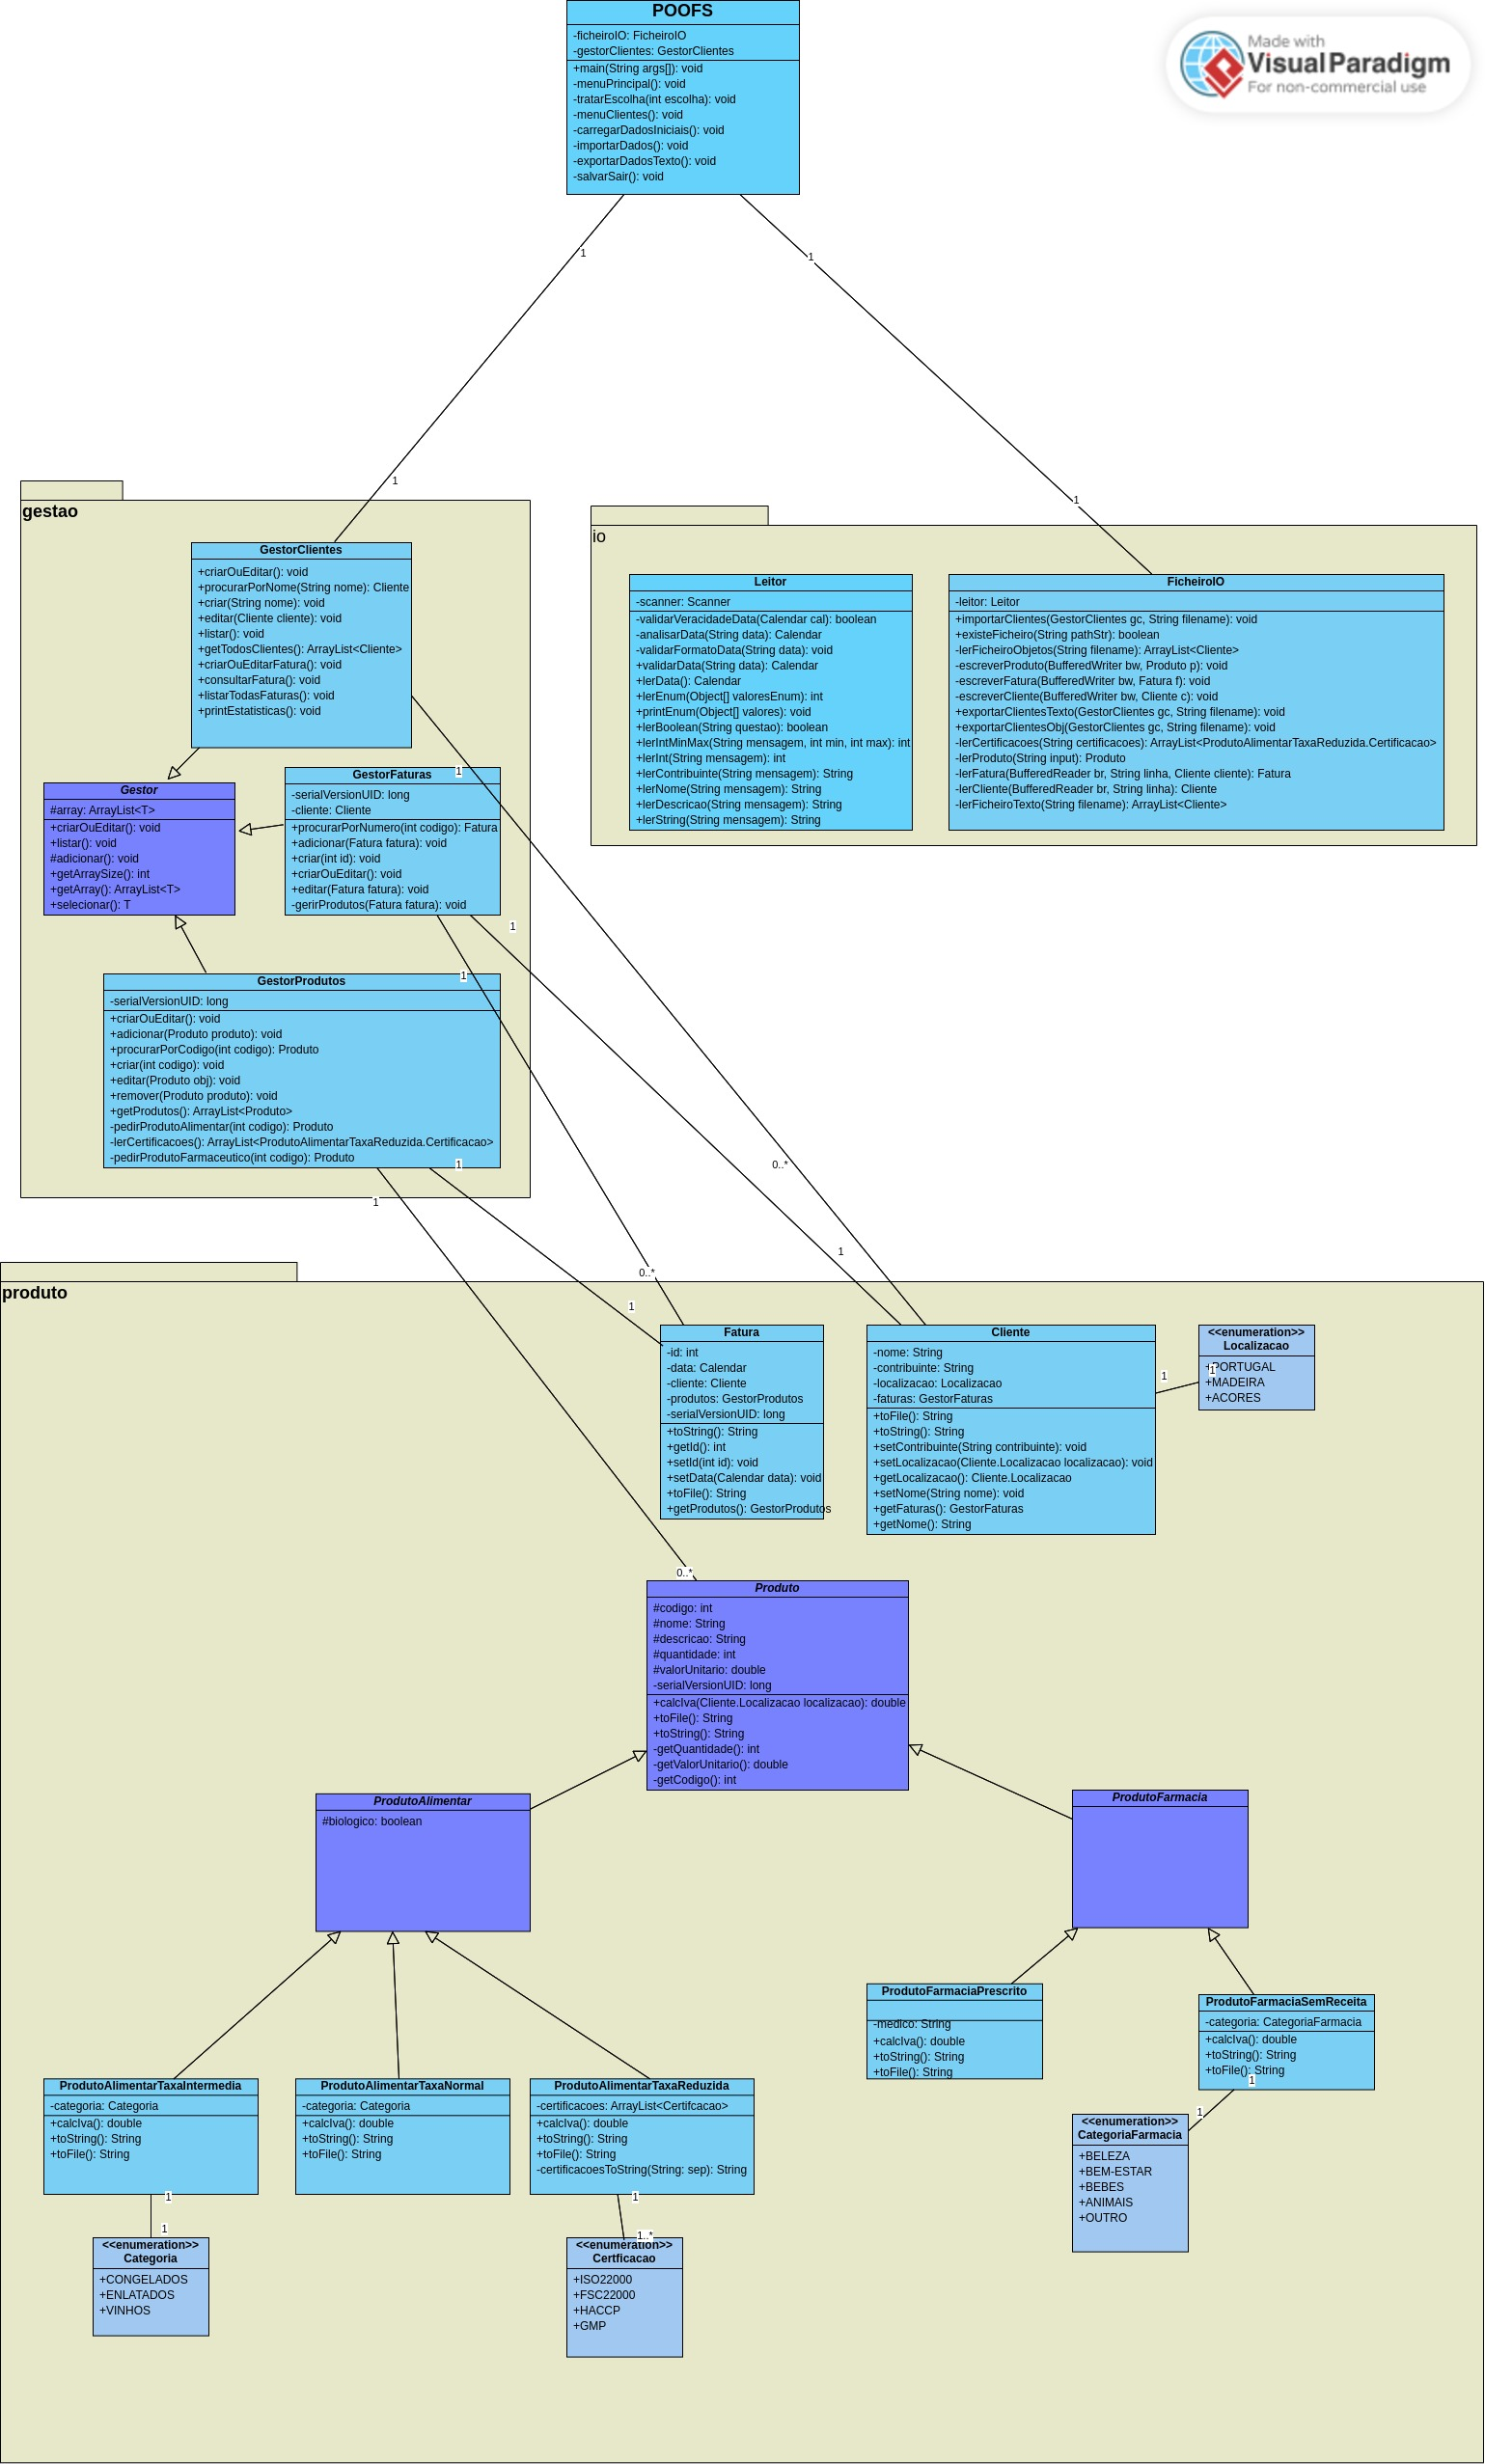
\includegraphics[width=0.45\textwidth]{uml-2} }}%
    \caption{UML Projetado Vs. UML Final}%
\end{figure}

\ssection{Conclusão e Observações}

O programa \textbf{POOFS} (\textit{POO Financial Services}) foi concebido para ajudar empresas a organizar as suas operações financeiras. Ele regista clientes, cria faturas, e oferece dados detalhados de forma clara e prática.

\sssection{Principais Benefícios:}
\begin{itemize}
    \setlength\itemsep{0em}
    \item Menu intuitivo que permite gerir clientes e faturas com facilidade tal como obter informações especificas.
    \item Suporte para produtos alimentares e farmacêuticos, com cálculos automáticos de IVA.
    \item Exportação e importação de dados para segurança e partilha.
\end{itemize}

\sssection{Considerações Finais}
\begin{itemize}
    \item O sistema tem uma arquitetura bem estruturada, que facilita manutenção e melhorias futuras.
\end{itemize}



\newpage


\end{document}

